\chapter{Example}
\label{chp:example}

This example is about Google and Apple Pay. It explains how these two paying applications work and why it is done how it is done. \\
Before diving into the algorithm behind the paying methods, some terms should be explained.

\begin{description}
	\item [Payment Networks] are credit institutions which managing credit cards and the transfer from money. But also Paypal and VisaCheckout are payment Networks.
	\item [Token Service Provider] are providing a very secure environment to map credit card information to individual token. \cite{token-service-provider}
	\item [Secure Enclave] is the build in security chip in Apple devices. All keys are stored in here.
	\item [Secure Element] is also apple specific and is paired with the Secure Enclave via hardware in the factory. It is located in the NFC-Chip to emulate the credit card.
\end{description}

Apple Pay and Google Pay are similar but different in detail. Both have four main steps.

\begin{enumerate}
	\item Adding a card
	\item Initiate
	\item Authorize
	\item Finish
\end{enumerate}

\newpage

\section{Google Pay}
\label{chp:example:sec:googlePay}

Google Pay is using the process of tokenization \cite{tokenization} like a lot other mobile payment application and is standardized together with card issuer and token service provider (TSP).\\
\begin{figure}[h!]
	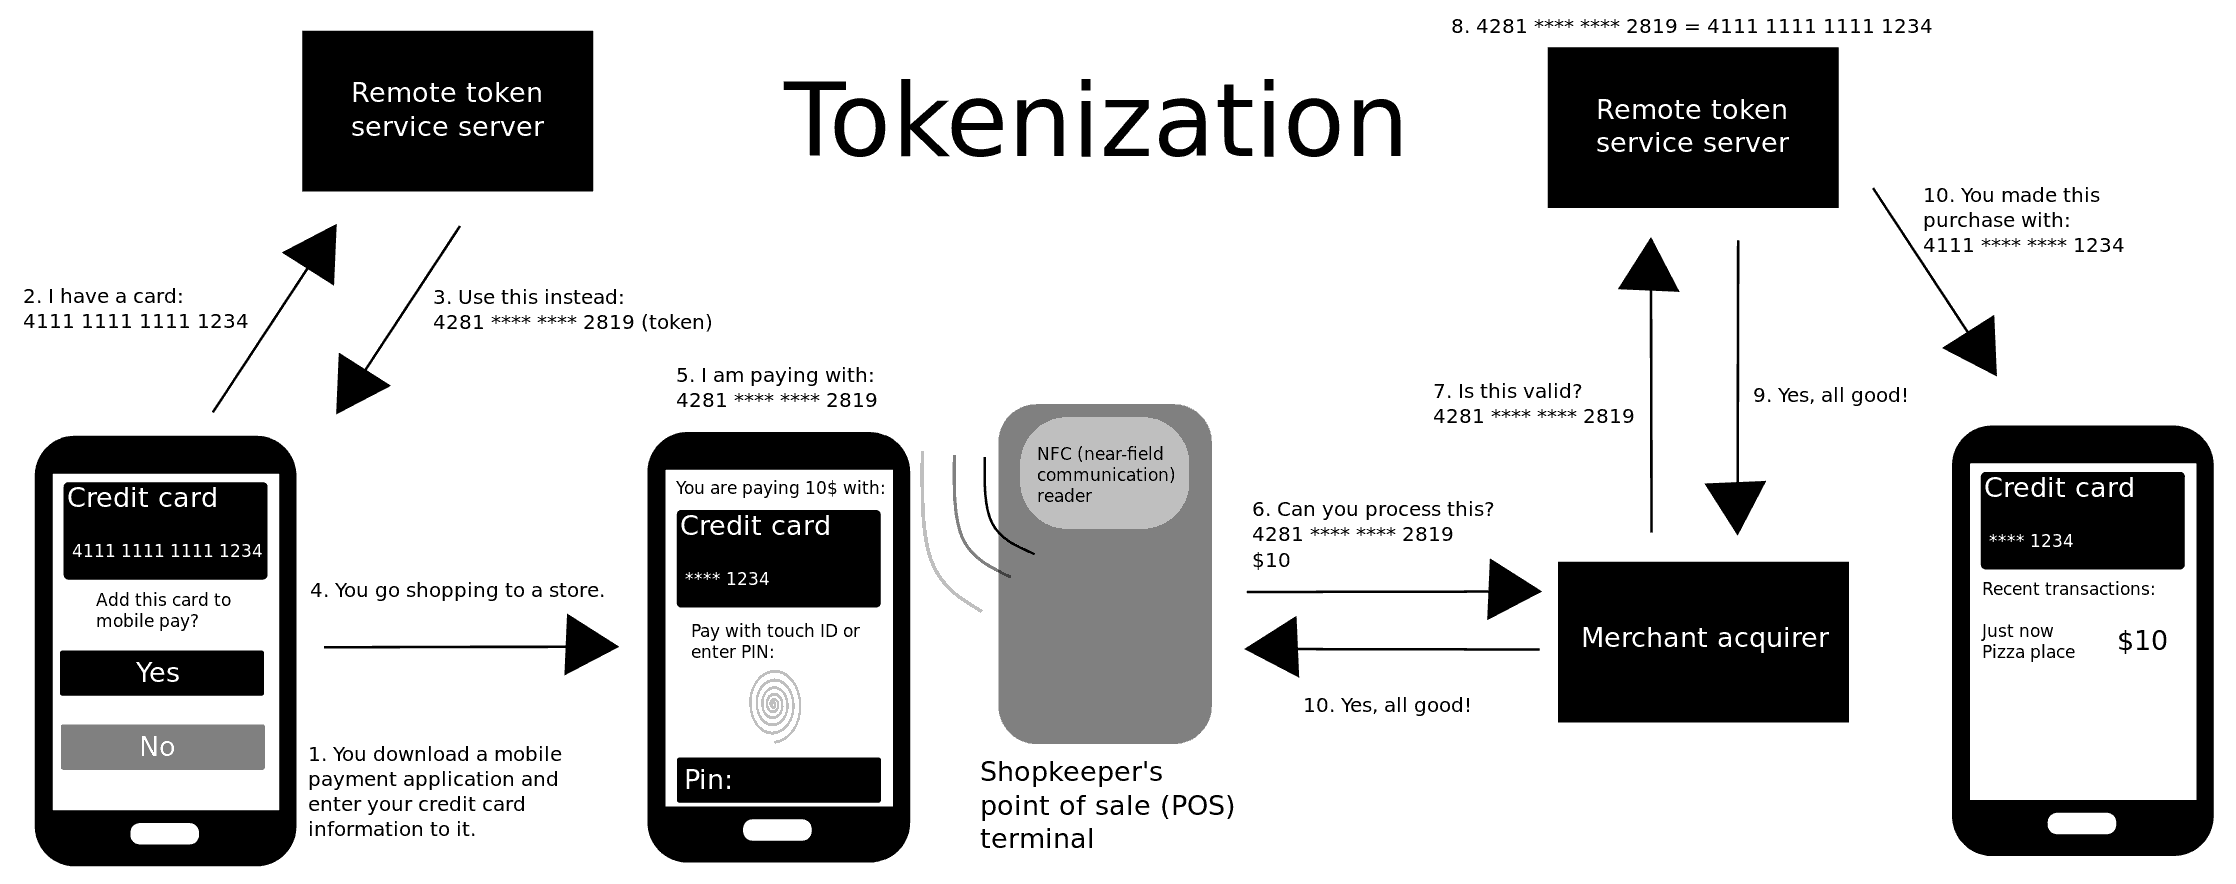
\includegraphics[width=\textwidth, angle=0]{How_mobile_payment_tokenization_works.png}
	\caption{Mobile payment tokenization}
	\label{img:mobile_payment_tokenization}
\end{figure}

\subsection{Adding a card}
\label{chp:example:sec:googlePay:ssec:addingACard}

After downloading the payment app (Fig. \ref{img:mobile_payment_tokenization} Step 1) the user gives the card number. In the background the app ask for a token to represent the card. (Fig. \ref{img:mobile_payment_tokenization} Step 2 and 3)\\
This token, provided from a TSP, is stored at the device and encrypted with a single or limited used key provided from the Payment Network. \\
This is an elegant way to not safe user data on the device. Security of the token is finally guaranteed by encryption. So this step applies two principles of security. 

\subsection{Initiate payment}
\label{chp:example:sec:googlePay:ssec:initiate}

The customers taps their device on a NFC Terminal (Fig. \ref{img:mobile_payment_tokenization} Step 4). With this action the application start transmitting the token, a token expire date and the cryptogram (Fig. \ref{img:mobile_payment_tokenization} Step 5). The cryptogram is generated by the token, timestamp and an Application Transaction Counter which is increased at every transaction and prevent the multiple use of one message.\\
This is a good example how appropriate protocols can be a secure way to communicate even if everybody could listen.\\

\subsection{Authorize}
\label{chp:example:sec:googlePay:ssec:authorize}

The merchant receive the message from NFC terminal and sends all information including the price to his card network (Fig. \ref{img:mobile_payment_tokenization} Step 6 and 7). The card network validates the cryptogram with help of TSP and matches the token to the real card number (Fig. \ref{img:mobile_payment_tokenization} Step 8).
\\
This step also fulfills one principle of security - validation.

\subsection{Finish}
\label{chp:example:sec:googlePay:ssec:finish}

Billing details get decrypted and the acquiring bank completes the transaction with customers bank Merchant and customer get information about validation (Fig. \ref{img:mobile_payment_tokenization} Step 9 and 10).\\ All with appropriated protocols. 
  